\documentclass{estilo}
\usepackage[spanish]{babel}
\usepackage{subcaption} % Debe ir en el preámbulo
\usepackage{dsfont}
\usepackage{graphicx}
\usepackage{float}
\usepackage{amsmath}        % para los vectores columnas
\usepackage{amsfonts}       % para las negrita de pizarra
\usepackage{amssymb}        % para simbolos matematicos
\usepackage{hyperref}       % para utilizar referencias
\usepackage{multirow}       % para las tablas
\usepackage{dsfont}
\usepackage{listings}
\usepackage{xcolor}
\definecolor{codegreen}{rgb}{0,0.6,0}
\definecolor{codegray}{rgb}{0.5,0.5,0.5}
\definecolor{codepurple}{rgb}{0.58,0,0.82}
\definecolor{backcolour}{rgb}{0.95,0.95,0.92}
\usepackage{chngcntr}
\counterwithin{figure}{section} % Esto hará que sea Figura 1.1, 2.1, 2.2, etc.

% Definición de colores mejorada
\definecolor{codegreen}{rgb}{0,0.6,0}
\definecolor{codegray}{rgb}{0.5,0.5,0.5}
\definecolor{codepurple}{rgb}{0.58,0,0.82}
\definecolor{backcolour}{rgb}{1,1,1} % Gris azulado muy tenue
\definecolor{keywordblue}{rgb}{0.13,0.29,0.53}


\lstdefinestyle{mystyle}{
    backgroundcolor=\color{backcolour},   
    commentstyle=\color{codegreen},
    keywordstyle=\color{keywordblue}\bfseries, % Azul oscuro para lógica
    numberstyle=\tiny\color{codegray},
    stringstyle=\color{codepurple},
    basicstyle=\ttfamily\footnotesize,
    breakatwhitespace=false,         
    breaklines=true,                 
    captionpos=b,                    
    keepspaces=true,                 
    numbers=left,                    
    numbersep=5pt,                  
    showspaces=false,                
    showstringspaces=false,
    showtabs=false,                  
    tabsize=2,
    frame=single,                           % Recuadro completo
    rulecolor=\color{gray!20},              % Color del borde suave
    % Definimos palabras clave personalizadas para tu algoritmo
    morekeywords={Si, Sino, Por, cada, en, devolver, Sea, el, inicializado, Ordenamos, por, mas, grande, al, chico}
}
\lstset{style=mystyle}

\usepackage{enumitem,multicol,setspace}
\newcounter{subenum}[enumi] % para las multicolumnas
\renewcommand{\thesubenum}{\arabic{subenum}}
\usepackage[nomessages]{fp}
\FPeval\thecolwidth{round(1/4:4)}% Specify number of columns -> column width
\newcommand{\newitem}[1]{%
  \refstepcounter{subenum}%
  \parbox{\dimexpr\thecolwidth\linewidth-.5\columnsep}{%
    \makebox[\labelwidth][r]{(\thesubenum)\hspace*{\labelsep}}%
    #1}\hfill%
}

\usepackage{scalerel,stackengine} % para el sombrero
\stackMath
\newcommand\rhat[1]{%
\savestack{\tmpbox}{\stretchto{%
  \scaleto{%
    \scalerel*[\widthof{\ensuremath{#1}}]{\kern-.6pt\bigwedge\kern-.6pt}%
    {\rule[-\textheight/2]{1ex}{\textheight}}%WIDTH-LIMITED BIG WEDGE
  }{\textheight}% 
}{0.5ex}}%
\stackon[1pt]{#1}{\tmpbox}%
}
\parskip 1ex

\usepackage{mathtools}      % floor y ceil
\DeclarePairedDelimiter\ceil{\lceil}{\rceil}
\DeclarePairedDelimiter\floor{\lfloor}{\rfloor} 

\usepackage[style=authoryear-comp]{biblatex}

\usepackage{listings}
\lstdefinestyle{fileformat}{
  backgroundcolor=\color{lightgray},
  basicstyle=\ttfamily\small,
  frame=single,
  breaklines=true,
  columns=fullflexible
}

\begin{document}
\maketitle

\justifying{}

\newpage
\section{Consideraciones}

En este trabajo practico, vamos a estar resolviendo el problema de Scaloni para  definir los días que deba entrenarse y los días que convenga descansar de tal forma de tener la mayor ganancia posible para los posibles N entrenamientos.


Para realizarlo, definimos la siguiente nomenclatura: 

\begin{itemize}
    \item El esfuerzo que demanda el dia i-ésimo es $e_i$, a su vez, esta es la ganancia maxima para ese dia.
    \item La energia por dia consecutivo disponible en el dia i-esimo viene definida por $s_i$
    \item Para cada dia $s_i$ (con $1 <= i <= N$) : $s_1 >= s_2 >= s_3 >= ... >= s_N$. 
    \item Tenemos N dias de de esfuerzo al igual que tenemos N dias de entrenamiento consecutivos.
\end{itemize}
\newpage
\justifying{
\hypertarget{res}{\section*{Ejemplo de Resolución}}
\section{Análisis del Problema}

El problema presenta una serie de decisiones secuenciales donde cada día $i$ el equipo técnico debe elegir entre dos opciones mutuamente excluyentes: \textbf{entrenar} o \textbf{descansar}. 

Sabemos que la ganancia de un entrenamiento no es estática, sino que depende directamente de la fatiga acumulada del plantel. Podemos expresar la ganancia de entrenar un día específico $j$, habiendo entrenado ininterrumpidamente desde un día $i$ (es decir, llevando $j-i+1$ días de fatiga), mediante la siguiente expresión matemática:

\begin{eqnarray}
g(i, j) = \min(e_j, s_{j-i+1})
\label{ganancia-diaria}
\end{eqnarray}

en donde $e_j$ es la expectativa de esfuerzo del día $j$, y $s$ representa el arreglo de energía disponible del equipo, el cual decrece a medida que aumentan los días consecutivos de entrenamiento.

\subsection{Matriz de Ganancias}

Para evitar recalcular las sumatorias de energía repetidas veces y aislar el concepto de ``días consecutivos'', introducimos una matriz de ganancias $\text{Ganancias}(i, j)$. Esta estructura almacena la ganancia total obtenida si el equipo entrena de forma ininterrumpida desde el día $i$ hasta el día $j$.

Debido a que la ganancia es acumulativa, podemos definir la construcción de esta matriz de manera iterativa:

\begin{eqnarray}
\text{Ganancias}(i, j) = 
\begin{cases} 
0 & \text{si } j < i \\
\text{Ganancias}(i, j-1) + \min(e_j, s_{j-i+1}) & \text{si } j \geq i
\end{cases}
\label{matriz-Ganancias}
\end{eqnarray}

Esta precomputación resulta en una matriz triangular superior que se puede construir en tiempo $\mathcal{O}(n^2)$, y nos permite consultar la ganancia de cualquier racha de entrenamientos en tiempo constante $\mathcal{O}(1)$.

\subsection{Ejemplo de la Matriz de Ganancias}

Para ilustrar la construcción y el significado de la matriz $\text{Ganancias}(i, j)$, consideremos un caso de ejemplo con $n=4$ días, donde los arreglos de esfuerzo esperado y energía disponible son:
\begin{itemize}
    \item Esfuerzo ($e$): $[10, 5, 12, 9]$
    \item Energía ($s$): $[15, 7, 5, 2]$
\end{itemize}

En la estructura de esta matriz:
\begin{itemize}
    \item Las \textbf{filas ($i$)} representan el \textbf{día de inicio} del bloque de entrenamiento ininterrumpido.
    \item Las \textbf{columnas ($j$)} representan el \textbf{día de finalización} de ese mismo bloque.
    \item Cada \textbf{celda} contiene la ganancia total acumulada si el equipo sale a entrenar todos los días en ese rango $[i, j]$.
\end{itemize}

Calculamos los primeros valores paso a paso aplicando la ecuación \eqref{matriz-Ganancias}:

\begin{itemize}
    \item \textbf{Fila 1 (Entrenamientos que empiezan el Día 1):} Arrancamos con la energía al máximo ($s_1 = 15$).
    \begin{itemize}
        \item $j=1$ (Entrenar solo D1): $\min(e_1, s_1) = \min(10, 15) = \mathbf{10}$
        \item $j=2$ (Entrenar D1 y D2): $\text{Ganancias}(1, 1) + \min(e_2, s_2) = 10 + \min(5, 7) = 10 + 5 = \mathbf{15}$
        \item $j=3$ (Entrenar D1 al D3): $\text{Ganancias}(1, 2) + \min(e_3, s_3) = 15 + \min(12, 5) = 15 + 5 = \mathbf{20}$
    \end{itemize}
    \item \textbf{Fila 2 (Entrenamientos que empiezan el Día 2):} Como asumimos que empezó el Día 2, la fatiga se resetea y usamos $s_1$ para el primer día de este bloque.
    \begin{itemize}
        \item $j=2$ (Entrenar solo D2): $\min(e_2, s_1) = \min(5, 15) = \mathbf{5}$
        \item $j=3$ (Entrenar D2 y D3): $\text{Ganancias}(2, 2) + \min(e_3, s_2) = 5 + \min(12, 7) = 5 + 7 = \mathbf{12}$
    \end{itemize}
\end{itemize}

Al completar todos los cálculos, la matriz resultante queda de la siguiente manera:

\begin{table}[h]
\centering
\begin{tabular}{|c|c|c|c|c|}
\hline
\textbf{Inicio ($i$) \textbackslash{} Fin ($j$)} & \textbf{$j=1$} & \textbf{$j=2$} & \textbf{$j=3$} & \textbf{$j=4$} \\ \hline
\textbf{$i=1$} & 10 & 15 & 20 & 22 \\ \hline
\textbf{$i=2$} & -  & 5  & 12 & 17 \\ \hline
\textbf{$i=3$} & -  & -  & 12 & 19 \\ \hline
\textbf{$i=4$} & -  & -  & -  & 9  \\ \hline
\end{tabular}
\caption{Matriz de Ganancias precomputada para $n=4$.}
\label{tabla-ganancias}
\end{table}

Por ejemplo, si observamos la celda en la fila $i=2$ y columna $j=4$, el valor $17$ representa explícitamente la ganancia obtenida si el equipo decide descansar el día 1, y luego entrena ininterrumpidamente durante los días 2, 3 y 4. Las celdas vacías debajo de la diagonal no son válidas matemáticamente, ya que un bloque de entrenamiento no puede terminar en un día anterior al que empezó.

\subsection{Ecuación de Recurrencia (1D)}

Con la matriz de ganancias definida, podemos modelar el problema principal utilizando Programación Dinámica. Definimos nuestro arreglo unidimensional de subproblemas $OPT(i)$ como \textit{``la ganancia máxima posible considerando únicamente los primeros $i$ días del torneo''}.

Para entender la lógica detrás de la ecuación, imaginemos que estamos parados en el día $i$ y queremos evaluar cómo maximizar nuestra ganancia acumulada hasta hoy. En lugar de preguntarnos si hoy entrenamos o descansamos, el algoritmo cambia el enfoque y se pregunta: \textbf{¿De qué tamaño será la racha ininterrumpida de entrenamientos que finaliza exactamente hoy?}

Si llamamos $k$ a la longitud de esa racha final de entrenamientos, el algoritmo evalúa exhaustivamente todas las opciones físicamente posibles (desde $k=1$ hasta $k=i$) y se queda con la que otorgue el mayor puntaje. Al evaluar cada $k$, el problema se divide en dos escenarios:

\begin{itemize}
    \item \textbf{Escenario de Racha Total ($k=i$):} 
    Significa que la decisión a evaluar es si conviene que el equipo haya entrenado todos los días de corrido desde que empezó el torneo hasta el día de hoy, sin descansar nunca. Como no hay días previos, la ganancia de esta opción es directamente el bloque completo que ya precomputamos: $\text{Ganancias}(1, i)$.

    \item \textbf{Escenario de Racha Parcial ($1 \le k < i$):} 
    Significa que el equipo entrena los últimos $k$ días consecutivos (desde el día $i-k+1$ hasta el día $i$), pero \textbf{obligatoriamente descansó el día inmediatamente anterior} (el día $i-k$). 
\end{itemize}

Al asumir que el día $i-k$ fue un día de descanso, sabemos que la fatiga del equipo se reseteó a cero. Por lo tanto, el puntaje total de esta opción será la suma de la ganancia de la nueva racha actual de $k$ días, más la \textbf{mejor historia posible} que el equipo haya podido construir en los días previos a ese descanso. 

Esa "mejor historia pasada" (que abarca desde el día $1$ hasta el día $i-k-1$) ya fue resuelta por el algoritmo en iteraciones anteriores y está guardada en $OPT(i-k-1)$.

Al unificar esta lógica matemática, formalizamos la ecuación evaluando de forma independiente la racha total para evitar acceder a índices negativos o inválidos en el arreglo $OPT$:

\begin{eqnarray}
OPT(i) = \max 
\begin{cases} 
\text{Ganancias}(1, i) & \text{(Racha total sin descansos)} \\
\max_{\forall\, k \in \{1,\dots,i-1\}} \Big( OPT(i - k - 1) + \text{Ganancias}(i-k+1, i) \Big) & \text{(Rachas parciales con descanso previo)}
\end{cases}
\label{ecuacion-recurrencia}
\end{eqnarray}

\subsection{Ejemplo del Cálculo de Óptimos ($OPT$)}

Continuando con nuestro ejemplo de $n=4$ días y utilizando la matriz de la Tabla \ref{tabla-ganancias}, evaluaremos el arreglo de óptimos $OPT$ aplicando la ecuación \eqref{ecuacion-recurrencia} de forma ascendente (\textit{bottom-up}), recordando que asumimos $OPT(0) = 0$.

\begin{itemize}
    \item \textbf{Día 1 ($i=1$):} 
    La única opción válida es entrenar desde el inicio ($k=1$).
    \begin{itemize}
        \item $OPT(1) = \text{Ganancias}(1, 1) = \mathbf{10}$. \textit{(Guardamos $k=1$)}.
    \end{itemize}

    \item \textbf{Día 2 ($i=2$):} 
    Evaluamos los posibles cortes $k$:
    \begin{itemize}
        \item Entrenar D1 y D2 ($k=2$): $\text{Ganancias}(1, 2) = \mathbf{15}$.
        \item Descansar D1, entrenar D2 ($k=1$): $OPT(0) + \text{Ganancias}(2, 2) = 0 + 5 = 5$.
        \item El máximo es $\mathbf{15}$. \textit{(Guardamos $k=2$)}.
    \end{itemize}

    \item \textbf{Día 3 ($i=3$):} 
    Evaluamos los posibles cortes $k$:
    \begin{itemize}
        \item Entrenar D1 al D3 ($k=3$): $\text{Ganancias}(1, 3) = 20$.
        \item Descansar D1, entrenar D2 y D3 ($k=2$): $OPT(0) + \text{Ganancias}(2, 3) = 0 + 12 = 12$.
        \item Descansar D2, entrenar D3 ($k=1$): $OPT(1) + \text{Ganancias}(3, 3) = 10 + 12 = \mathbf{22}$.
        \item El máximo es $\mathbf{22}$. \textit{(Guardamos $k=1$)}.
    \end{itemize}

    \item \textbf{Día 4 ($i=4$):} 
    Evaluamos los posibles cortes $k$:
    \begin{itemize}
        \item Entrenar D1 al D4 ($k=4$): $\text{Ganancias}(1, 4) = 22$.
        \item Descansar D1, entrenar D2 al D4 ($k=3$): $OPT(0) + \text{Ganancias}(2, 4) = 0 + 17 = 17$.
        \item Descansar D2, entrenar D3 y D4 ($k=2$): $OPT(1) + \text{Ganancias}(3, 4) = 10 + 19 = \mathbf{29}$.
        \item Descansar D3, entrenar D4 ($k=1$): $OPT(2) + \text{Ganancias}(4, 4) = 15 + 9 = 24$.
        \item El máximo absoluto del problema es $\mathbf{29}$. \textit{(Guardamos $k=2$)}.
    \end{itemize}
\end{itemize}

El arreglo final resulta ser $OPT = [10, 15, 22, 29]$. El valor $OPT(4) = 29$ representa la máxima ganancia posible para todo el torneo.

\subsection{Complejidad y Reconstrucción}

La solución planteada requiere dos fases. En primer lugar, la construcción de la matriz $\text{Ganancias}(i, j)$ toma tiempo $\mathcal{O}(n^2)$ y espacio $\mathcal{O}(n^2)$. 

En segundo lugar, el cálculo del arreglo unidimensional $OPT$ de tamaño $n$ requiere iterar $i$ desde $1$ hasta $n$, y en el peor de los casos, el bucle interno de maximización evalúa $i-1$ cortes posibles. Esto resulta en una sumatoria de Gauss, la cual también se acota en tiempo $\mathcal{O}(n^2)$.

El resultado óptimo del problema se encontrará en la última posición del arreglo, $OPT(n)$. 

Para reducir la complejidad de reconstruir el cronograma de entrenamientos (camino óptimo), se va a almacenar el valor del $k$ final para poder reconstruir cada paso en $\mathcal{O}(1)$, mejorando la reconstrucción a $\mathcal{O}(n)$. Basta con realizar un proceso de \textit{backtracking} desde $OPT(n)$, con el último $k$ obtenido, marcando esos $k$ días como entrenamiento, el día anterior como descanso $(i-k)$, y saltando recursivamente al estado del día anterior $OPT(i-k-1)$, así sucesivamente hasta llegar al inicio (top-down).
\section{Solución propuesta}

Luego de lo mencionado anteriormente presentamos un pseudocodigo que muestra la solución propuesta por programación dinámica para este problema

\begin{figure}[H]
\centering
\begin{lstlisting}[style=fileformat]
Entrenamientos(e,s): 

	Sea N igual al largo de e o s mas 1
	Sea g una matriz de NxN con todos ceros
	Sea k un entero iniciado en 0
	Sea opt un arreglo de largo N inicializado con 0s
	
	Por cada i entre 1 a N:
		Por cada j entre 1 a N:
			Si i>j: 
				continuamos 
			Si j == i:
				g[i][j]=e[i]
			Sino:
				g[i][j]= g[i][j-1] + min(e[j],s[j-i])
	
	Por cada i entre 1 a N:
		Sea opt_k un arreglo de largo N inicializado en 0s
		Sea mayor_opt un entero inicializado en 0
			
		Por cada j entre 1 a i:
			Si j != i:
				opt_k[j] = opt[i-j-1]+g[i-j+1][i]
			Sino:
				opt_k[j] = g[1][j]
			
			Si opt_k[j]>=mayor_opt:
				mayor_opt = opt_k[j]
				k=j
		opt[i] = opt_k[k]

	devolver reconstruccion(opt, k)	
	
\end{lstlisting}
\label{cod:ordenado}
\caption{Pseudocodigó propuesto para resolver el problema}
\end{figure}


Siendo reconstrucción el algoritmo de para obtener la solución, que se vuelve mas simple guardando el ultimo k. Este algoritmo corresponde al siguiente pseudocodigo

\begin{figure}[H]
\centering
\begin{lstlisting}[style=fileformat]
Reconstruccion(opt,k): 

	Sea dia el calculo de len(opt)-1-k
	Por cada i entre 0 a k
		

    Sea rec una lista vacia con la solcuion
    Mientras len(rec) < len(opt):
         Sea dia igual a len(opt)-1 -k -1
         Por cada i entre 0 a k
            agregamos 'E' a rec
         agregamos 'D' a rec
         k=dia

    Damos vuelta la lista rec
    Borramos la primera componente que es la componente 'D' agregada al final
	Devolvemos rec

\end{lstlisting}
\label{cod:ordenado}
\caption{Pseudocodigó propuesto para reconstruir la solucion}
\end{figure}
%\section*{Demostración de Optimalidad: Algoritmo Greedy}

Para demostrar que nuestra estrategia Greedy (ordenar los videos de forma descendente según el tiempo del ayudante $a_i$) es óptima, utilizaremos método de inversiones.

\subsection*{Definiciones}
Sea $S$ un conjunto de $n$ rivales a analizar. Para cada rival $i$, definimos:
\begin{itemize}
    \item $s_i$: Tiempo que le toma a Scaloni analizar el rival $i$.
    \item $a_i$: Tiempo que le toma al ayudante analizar el rival $i$.
\end{itemize}
El tiempo de finalización de un rival $i$ depende de la suma de los tiempos de Scaloni de todos los rivales anteriores, más $s_i$ y $a_i$. El objetivo es minimizar el tiempo máximo en el que terminan los ayudantes y Scaloni.

\subsection*{Hipótesis}
Nuestra solución Greedy se basa en ordenar de forma descendente a los pares ($s_i$, $a_i$), de forma tal que los primeros rivales a ser analizados son los que tienen mayor tiempo de análisis por ayudante. Es importante recalcar que el análisis de los rivales se produce sin tiempo de desuso. Se espera que con esta estrategia de ordenamiento, el tiempo máximo en el que Scaloni y sus ayudantes pueden analizar a todos sus rivales sea el mínimo. 

Por lo tanto, para cada par de rivales en nuestra solución propuesta es:

$$a_i > a_j > ... > a_n$$


Vamos a probar que la solución Greedy da siempre un orden óptimo utilizando el método de inversiones.


\subsection*{Definición de Inversión}
Supongamos que existe un algoritmo $O$ óptimo distinto a la solución Greedy propuesta. Si $O$ tiene una inversión, entonces existe un par de rivales a procesar $i$ y $j$ en el que $j$ fue analizado inmediatamente después de $i$ (primero $i$, luego $j$) de tal forma que presentan una inversión respecto a la regla Greedy:
$$a_i < a_j$$
Supongamos que Scaloni comienza a analizar el rival $i$ en un tiempo acumulado $T$. 

\newpage

\subsection*{Análisis del Cronograma Óptimo $O$}
Los tiempos de finalización para este par de tareas en $O$ son:
\begin{itemize}
    \item El ayudante termina el rival $i$ en: $C_i = T + s_i + a_i$
    \item El ayudante termina el rival $j$ en: $C_j = T + s_i + s_j + a_j$
\end{itemize}
El tiempo máximo para este bloque en $O$ es el máximo entre $C_i$ y $C_j$. Como $s_j > 0$ y por nuestra hipótesis de inversión $a_j > a_i$, es evidente que:
$$\text{Max}_{O} = \max(T + s_i + a_i, \, T + s_i + s_j + a_j) = T + s_i + s_j + a_j$$

\subsection*{El Intercambio (Cronograma $O'$)}
Construimos un nuevo cronograma $O'$ intercambiando únicamente el orden de $i$ y $j$ (primero $j$, luego $i$), dejando el resto intacto. Los nuevos tiempos de finalización son:
\begin{itemize}
    \item El ayudante termina el rival $j$ en: $C'_j = T + s_j + a_j$
    \item El ayudante termina el rival $i$ en: $C'_i = T + s_j + s_i + a_i$
\end{itemize}
El tiempo máximo para este bloque en el nuevo cronograma $O'$ es:
$$\text{Max}_{O'} = \max(T + s_j + a_j, \, T + s_j + s_i + a_i)$$

\subsection*{Comparación de optimalidad}
Comparamos ambos términos de $\text{Max}_{O'}$ con $\text{Max}_{O}$:
\begin{enumerate}
    \item $T + s_j + a_j < T + s_i + s_j + a_j$ (ya que $s_i > 0$).
    \item $T + s_j + s_i + a_i < T + s_i + s_j + a_j$ (ya que $a_i < a_j$ por la inversión).
\end{enumerate}

Ambos tiempos posibles de finalización en $O'$ son estrictamente menores al tiempo de finalización en $O$. Además, como ambos rivales en conjunto siguen consumiendo exactamente $s_i + s_j$ del tiempo de Scaloni, el tiempo de inicio de todos los rivales posteriores no se ve afectado.

Por lo tanto, el \textit{tiempo máximo} de $O'$ es menor o igual al de $O$. Como $O$ era óptimo, $O'$ también debe serlo. Repitiendo este proceso para deshacer cada inversión, llegaremos exactamente a nuestro ordenamiento Greedy sin aumentar el tiempo total. 

Esto explica matemáticamente por qué el tiempo global de nuestro nuevo cronograma $O'$ será \textbf{menor o igual} ($\le$) al de $O$. Pueden existir configuraciones óptimas con inversiones inofensivas que no penalizan el tiempo global, pero el intercambio demuestra rigurosamente que llevar cualquier configuración a su forma Greedy jamás empeorará el resultado. $\blacksquare$

\newpage

\subsection*{Análisis de Múltiples Óptimos y Tiempo Global}
Es fundamental notar la diferencia entre el tiempo máximo \textit{local} del bloque intercambiado y el tiempo de finalización \textit{global} de todo el proyecto. 

Supongamos un escenario genérico donde existe una tarea inicial tan demandante para un ayudante que define, por sí sola, el tiempo de finalización de todo el proyecto (un gran cuello de botella). Si más adelante en el cronograma existe un par de tareas invertidas (una corta seguida de una más larga), deshacer esa inversión mejorará estrictamente el tiempo \textit{local} de ese par. Sin embargo, como el tiempo de ese pequeño bloque queda ``oculto'' o absorbido por la larga espera de la tarea gigante inicial, el tiempo \textit{global} del proyecto se mantendrá exactamente igual.

\begin{figure}[H]
    \centering
    \begin{tikzpicture}[x=0.8cm, y=0.7cm]
        
        % ==========================================
        % CRONOGRAMA 1: Óptimo (Con Inversión)
        % ==========================================
        \node[anchor=east, font=\bfseries] at (-1, 0) {Óptimo (Con Inversión)};
        
        % Eje Scaloni
        \node[anchor=east] at (0, -1) {Scaloni:};
        \draw[fill=gray!30] (0,-1.4) rectangle (1,-0.6) node[midway] {$s_1$};
        \draw[fill=red!30]  (1,-1.4) rectangle (2,-0.6) node[midway] {$s_i$};
        \draw[fill=blue!30] (2,-1.4) rectangle (3,-0.6) node[midway] {$s_j$};
        \draw[fill=green!30](3,-1.4) rectangle (4,-0.6) node[midway] {$s_k$};
        
        % Ejes Ayudantes
        \node[anchor=east] at (0, -2.5) {Ayudantes:};
        % Ayudante 1
        \draw[fill=gray!30] (1,-2.9) rectangle (11,-2.1) node[midway] {$a_1$};
        % Ayudante x
        \draw[fill=red!30]  (2,-3.9) rectangle (6,-3.1) node[midway] {$a_i$};
        % Ayudante y
        \draw[fill=blue!30] (3,-4.9) rectangle (8,-4.1) node[midway] {$a_j$};
        % Ayudante z
        \draw[fill=green!30](4,-5.9) rectangle (6,-5.1) node[midway] {$a_k$};

        % Línea de Tiempo Máximo
        \draw[dashed, thick] (11, 0) -- (11, -14) node[pos=0.1, right] {$T_{\max}$ Global};

        \node[anchor=west, text width=10cm, font=\small, text=black!70] at (0, -7) {
            \textbf{Observación:} Óptimo con inversion donde $a_i < a_j$.
        };

        % ==========================================
        % CRONOGRAMA 2: Greedy (Sin Inversión)
        % ==========================================
        \node[anchor=east, font=\bfseries] at (-1, -8) {Greedy (Sin Inversión)};
        
        % Eje Scaloni
        \node[anchor=east] at (0, -9) {Scaloni:};
        \draw[fill=gray!30] (0,-9.4) rectangle (1,-8.6) node[midway] {$s_1$};
        \draw[fill=blue!30] (1,-9.4) rectangle (2,-8.6) node[midway] {$s_i$};
        \draw[fill=red!30]  (2,-9.4) rectangle (3,-8.6) node[midway] {$s_j$};
        \draw[fill=green!30](3,-9.4) rectangle (4,-8.6) node[midway] {$s_k$};
        
        % Ejes Ayudantes
        \node[anchor=east] at (0, -10.5) {Ayudantes:};
        % Ayudante 1
        \draw[fill=gray!30] (1,-10.9) rectangle (11,-10.1) node[midway] {$a_1$};
        % Ayudante y
        \draw[fill=blue!30] (2,-11.9) rectangle (7,-11.1) node[midway] {$a_j$};
        % Ayudante x
        \draw[fill=red!30]  (3,-12.9) rectangle (7,-12.1) node[midway] {$a_i$};
        % Ayudante z
        \draw[fill=green!30](4,-13.9) rectangle (6,-13.1) node[midway] {$a_k$};
        
        % Notas
        \node[anchor=west, text width=10cm, font=\small, text=black!70] at (0, -17) {
            \textbf{Observación visual:} Al deshacer la inversión e intercambiar $(s_i, a_i)$ por $(s_j, a_j)$, los tiempos locales de esos ayudantes cambian. Sin embargo, como el bloque $a_1$ es inmenso y se extiende mucho más a la derecha, la línea de corte global ($T_{\max}$) permanece exactamente en el mismo lugar. Esto demuestra que la inversión no afectaba el tiempo global, y resolverla no empeora la optimalidad.
        };

    \end{tikzpicture}
    \caption{Comparación visual de los cronogramas con y sin inversión. La tarea $(s_1, a_1)$ enmascara los tiempos locales de $(s_i, a_i)$ y $(s_j, a_j)$.}
    \label{fig:inversiones}
\end{figure}


\subsection*{Conclusión}
Como $O$ era óptimo y demostramos que el tiempo global de $O'$ es menor o igual, $O'$ también debe ser óptimo. Repitiendo este proceso de intercambio para deshacer cada inversión, llegaremos exactamente a nuestro ordenamiento Greedy sin aumentar el tiempo total en ningún paso. Se concluye que el algoritmo Greedy propuesto siempre pertenece al conjunto de soluciones óptimas, minimizando el tiempo global. $\blacksquare$

\section{Análisis de Variabilidad y Optimalidad}

A continuación, analizamos cómo la variabilidad de los parámetros de entrada afecta el comportamiento del algoritmo de Programación Dinámica, la optimalidad de la solución teórica y la posterior reconstrucción empírica del cronograma.

\subsection{Afectación de la variabilidad a la ganancia y optimalidad}

La variabilidad en las distribuciones de los valores de esfuerzo ($e$) y energía ($s$) \textbf{no afecta la optimalidad de la solución algorítmica}. Al evaluar exhaustivamente todos los tamaños de bloques posibles $k$ hacia atrás y apoyarse en subestructuras óptimas ya calculadas, la ecuación de recurrencia garantiza matemáticamente encontrar siempre la ganancia máxima absoluta, sin importar si los datos son uniformes, extremos o atípicos.

Sin embargo, la forma de estos arreglos \textbf{sí afecta drásticamente la estructura del cronograma óptimo resultante} y la cantidad de soluciones óptimas posibles. Analizamos en detalle distintos escenarios:

\begin{enumerate}
    \item \textbf{Caso A: Energía casi inagotable o constante.}
    \begin{itemize}
        \item \textbf{Descripción:} El arreglo de energía $s$ se mantiene en valores muy altos y decae sumamente lento, superando holgadamente a los valores de esfuerzo $e_i$ en la gran mayoría de los días.
        \item \textbf{Análisis:} En este escenario, la función de ganancia diaria $\min(e_j, s_{j-i+1})$ estará dominada exclusivamente por los valores de $e_j$. Dado que la energía no es un limitante, tomar un día de descanso implica sumar $0$ a la ganancia de ese día sin obtener un beneficio real a cambio para el futuro. Como resultado, el algoritmo tenderá a elegir bloques de tamaño máximo ($k=i$), construyendo un cronograma de entrenamiento continuo y sin interrupciones.
    \end{itemize}

    \begin{figure}[H]
        \centering
        \begin{tikzpicture}[x=1.8cm, y=0.8cm]
            \node[anchor=east, font=\bfseries] at (-0.5, 0.5) {Cronograma:};
            \draw[fill=blue!30] (0,0) rectangle (1,1) node[midway] {Entrenar};
            \draw[fill=blue!30] (1,0) rectangle (2,1) node[midway] {Entrenar};
            \draw[fill=blue!30] (2,0) rectangle (3,1) node[midway] {Entrenar};
            \draw[fill=blue!30] (3,0) rectangle (4,1) node[midway] {Entrenar};
            
            \node[below] at (0.5, 0) {Día 1};
            \node[below] at (1.5, 0) {Día 2};
            \node[below] at (2.5, 0) {Día 3};
            \node[below] at (3.5, 0) {Día 4};
            
            \draw[thick] (0,1.2) -- (0,1.4) -- (4,1.4) -- (4,1.2);
            \node[above] at (2, 1.4) {$s_j \gg e_i \rightarrow$ Ganancia máxima sin descansos ($k=4$)};
        \end{tikzpicture}
    \end{figure}

    \item \textbf{Caso B: Caída abrupta de energía.}
    \begin{itemize}
        \item \textbf{Descripción:} El equipo sufre de fatiga extrema muy rápido. Por ejemplo, la energía inicial $s_1$ tiene un valor alto, pero para el segundo día consecutivo ($s_2$) decae abruptamente a valores cercanos a $0$.
        \item \textbf{Análisis:} Si la energía se desploma al segundo día de entrenamiento, cualquier bloque de tamaño $k \ge 2$ sumará un valor marginal en sus últimos días. Al algoritmo le resultará matemáticamente mucho más rentable insertar un día de descanso para resetear la fatiga y volver a aprovechar el alto valor de $s_1$. En consecuencia, la estructura del cronograma será una secuencia fragmentada, alternando estrictamente días de entrenamiento cortos (bloques de $k=1$) con días de descanso.
    \end{itemize}

    \begin{figure}[H]
        \centering
        \begin{tikzpicture}[x=1.8cm, y=0.8cm]
            \node[anchor=east, font=\bfseries] at (-0.5, 0.5) {Cronograma:};
            \draw[fill=blue!30] (0,0) rectangle (1,1) node[midway] {Entrenar};
            \draw[fill=red!30]  (1,0) rectangle (2,1) node[midway] {Descansar};
            \draw[fill=blue!30] (2,0) rectangle (3,1) node[midway] {Entrenar};
            \draw[fill=red!30]  (3,0) rectangle (4,1) node[midway] {Descansar};
            
            \node[below] at (0.5, 0) {Día 1};
            \node[below] at (1.5, 0) {Día 2};
            \node[below] at (2.5, 0) {Día 3};
            \node[below] at (3.5, 0) {Día 4};
            
            \draw[thick] (0,1.2) -- (0,1.4) -- (4,1.4) -- (4,1.2);
            \node[above] at (2, 1.4) {$s_2 \approx 0 \rightarrow$ Reseteo constante de fatiga (bloques de $k=1$)};
        \end{tikzpicture}
    \end{figure}

\end{enumerate}

\subsection{Comportamiento en Programación Dinámica (Bottom-Up) vs. Reconstrucción (Top-Down)}

En contextos de alta variabilidad que generan empates sistemáticos (como en el Caso C), el impacto se debe interpretar de manera distinta según la fase del algoritmo:

\begin{itemize}
    \item \textbf{Fase Bottom-Up (Llenado del arreglo $OPT$):} La variabilidad y la multiplicidad de opciones \textbf{no afectan en lo absoluto el cálculo del valor óptimo}. Cuando la función $\max$ de la ecuación de recurrencia evalúa diferentes tamaños de bloque $k$ y descubre que varios devuelven el mismo puntaje máximo, la ecuación simplemente asimila ese número. El valor final acumulado que llegará a $OPT(n)$ será único, robusto y representará la ganancia teórica inamovible, a prueba de cualquier volatilidad en los datos de entrada.
    
    \item \textbf{Fase Top-Down (Algoritmo de Reconstrucción):} Aquí es donde la alta variabilidad tiene un impacto real y directo. Si durante la fase \textit{Bottom-Up} existieron múltiples valores de $k$ que empataron como el máximo para un mismo día $i$, significa que existen \textbf{múltiples cronogramas estructuralmente distintos que logran exactamente la misma ganancia total}. 
    
    Un algoritmo de reconstrucción típico almacena solo un valor de $k$ ganador por celda para lograr una complejidad de $\mathcal{O}(n)$. La decisión de \textit{cuál} $k$ se guarda ante un empate depende de un simple operador lógico en la implementación: si el código utiliza un comparador estricto ($>$), conservará el primer $k$ que encuentre; si utiliza mayor o igual ($\geq$), sobrescribirá la variable y se quedará con el último $k$ óptimo evaluado. 
    
    Por lo tanto, ante datos que generan empates constantes, el cronograma específico devuelto (el detalle de qué días puntuales se entrena o se descansa) puede variar diametralmente de una ejecución a otra o entre distintas implementaciones del mismo algoritmo, \textbf{aunque todas esas versiones representen caminos 100\% óptimos}.
\end{itemize}
%\section{Mediciones}

Como sabemos el código corre en un tiempo $O(n log n)$ pero para poder demostrar que el código en realidad demora dicho tiempo, vamos a estar realizando una medición sobre el algoritmo. 

El método de medición consiste en realizar un set de datos usando un código que genera una cantidad de datos igual al parámetro de entrada, es decir, si el parámetro de entrada es 10, va a generar un archivo \textit{10.txt} con 10 rivales. Si se pasa una lista de M valores, genera M archivo con dichos valores (el parámetro esta hardcodeado en el archivo python).

Luego, corremos el código en modo de medición usando el comando python tp1.py --medir (tener cuidado con el -- de latex, puede fallar al copiarlo directamente), el cual realiza la medición de los tiempos por cada uno de los archivos generados anteriormente y guarda el resultada en un archivo llamado \textit{mediciones.txt} con el siguiente formato: 

\begin{figure}[H]
\centering
\begin{lstlisting}[style=fileformat]
10,tiempo de n=10
100,tiempo de n=100
1000,tiempo de n=1000
....
N,tiempo de n=N
\end{lstlisting}
\label{cod:fileOrdenamiento}
\caption{Archivo mediciones.txt}
\end{figure}

en donde, cada fila indica el tiempo que demoro el algoritmo con la cantidad de N datos en el archivo. De esta forma vamos a poder graficar los resultados y aproximar dicho puntos usando el método de cuadrado mínimo.

La siguiente figura muestra la aproximacion de las funciones $O(n log n)$ y $O(n^2)$ viendo que los puntos se aproximan mejor a una función de $O(n log n)$ que al tiempo de $O(n^2)$, demostrando que la teoria es correcta. 

\begin{figure}[H]
    \centering
    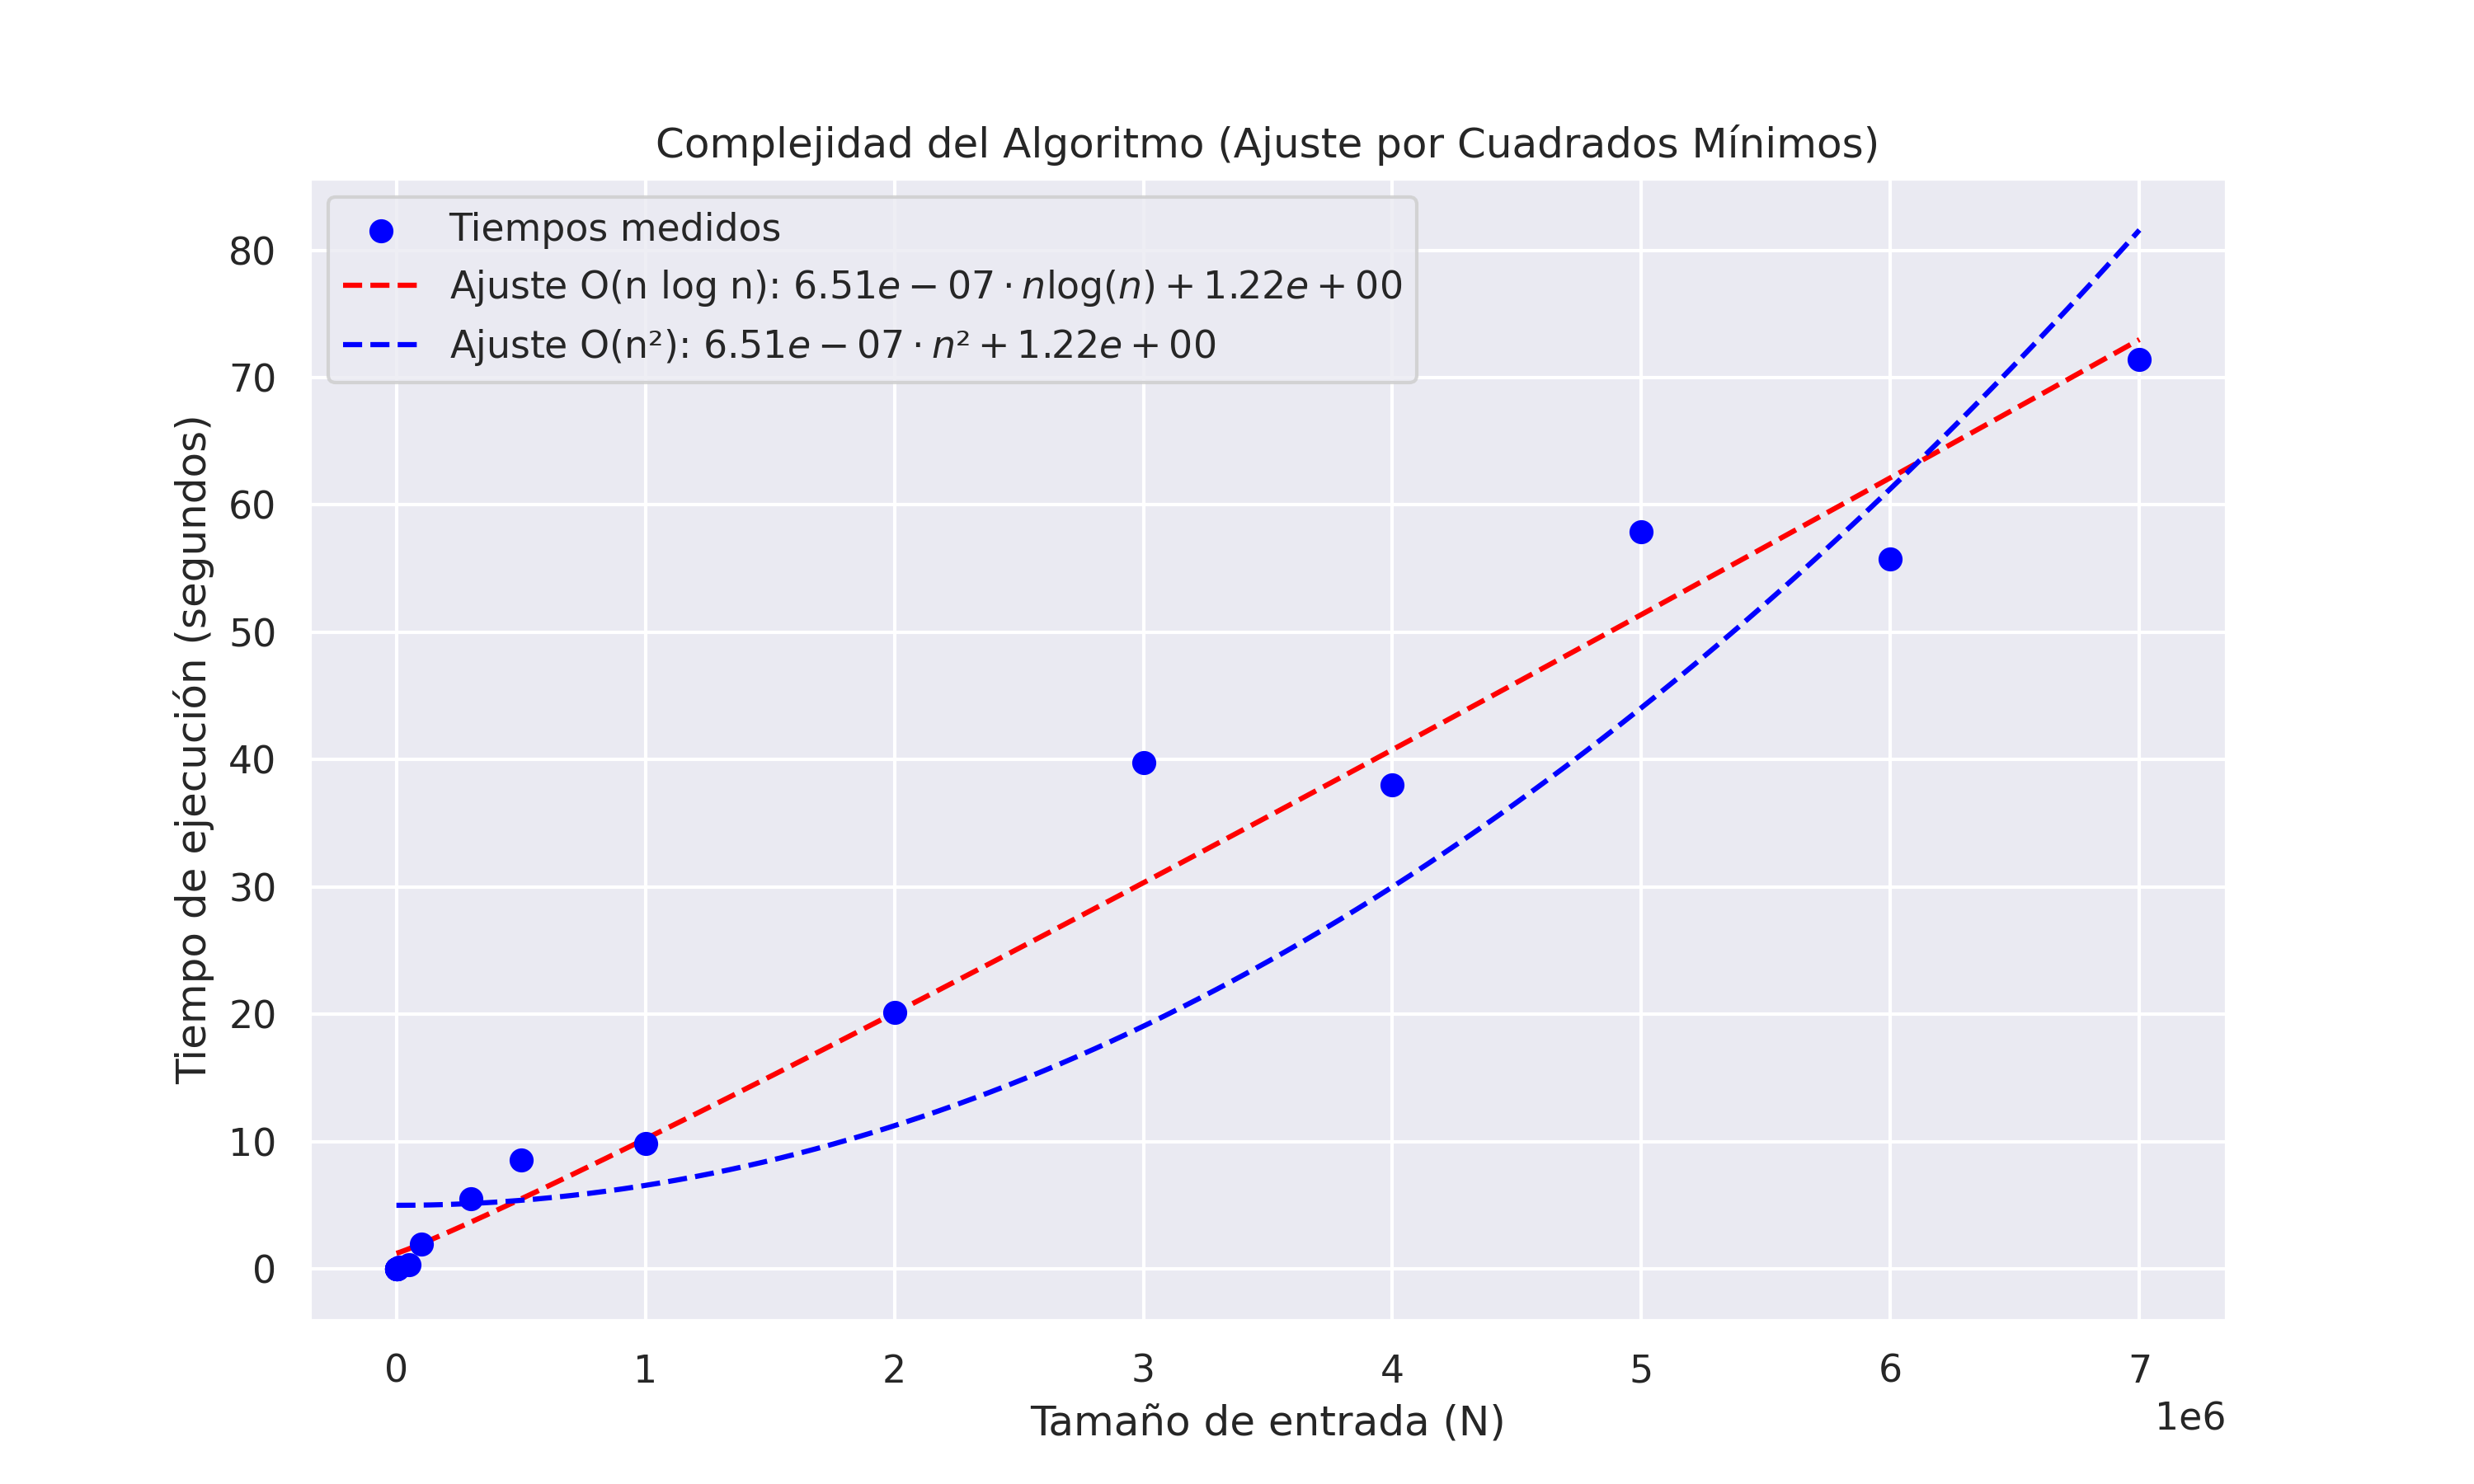
\includegraphics[width=1\textwidth]{img/tiempos.png}
\end{figure}

Es importante mostrar el error de la función aproximada con el teórico de esta forma podemos demostrar de una forma mas teórica a que función corresponde mas, demostrando que de forma teórica el error de la aproximación de $O(n log n)$  es menor al error de $O(n^2)$. Esto lo observamos en la siguiente figura.

\begin{figure}[H]
    \centering
    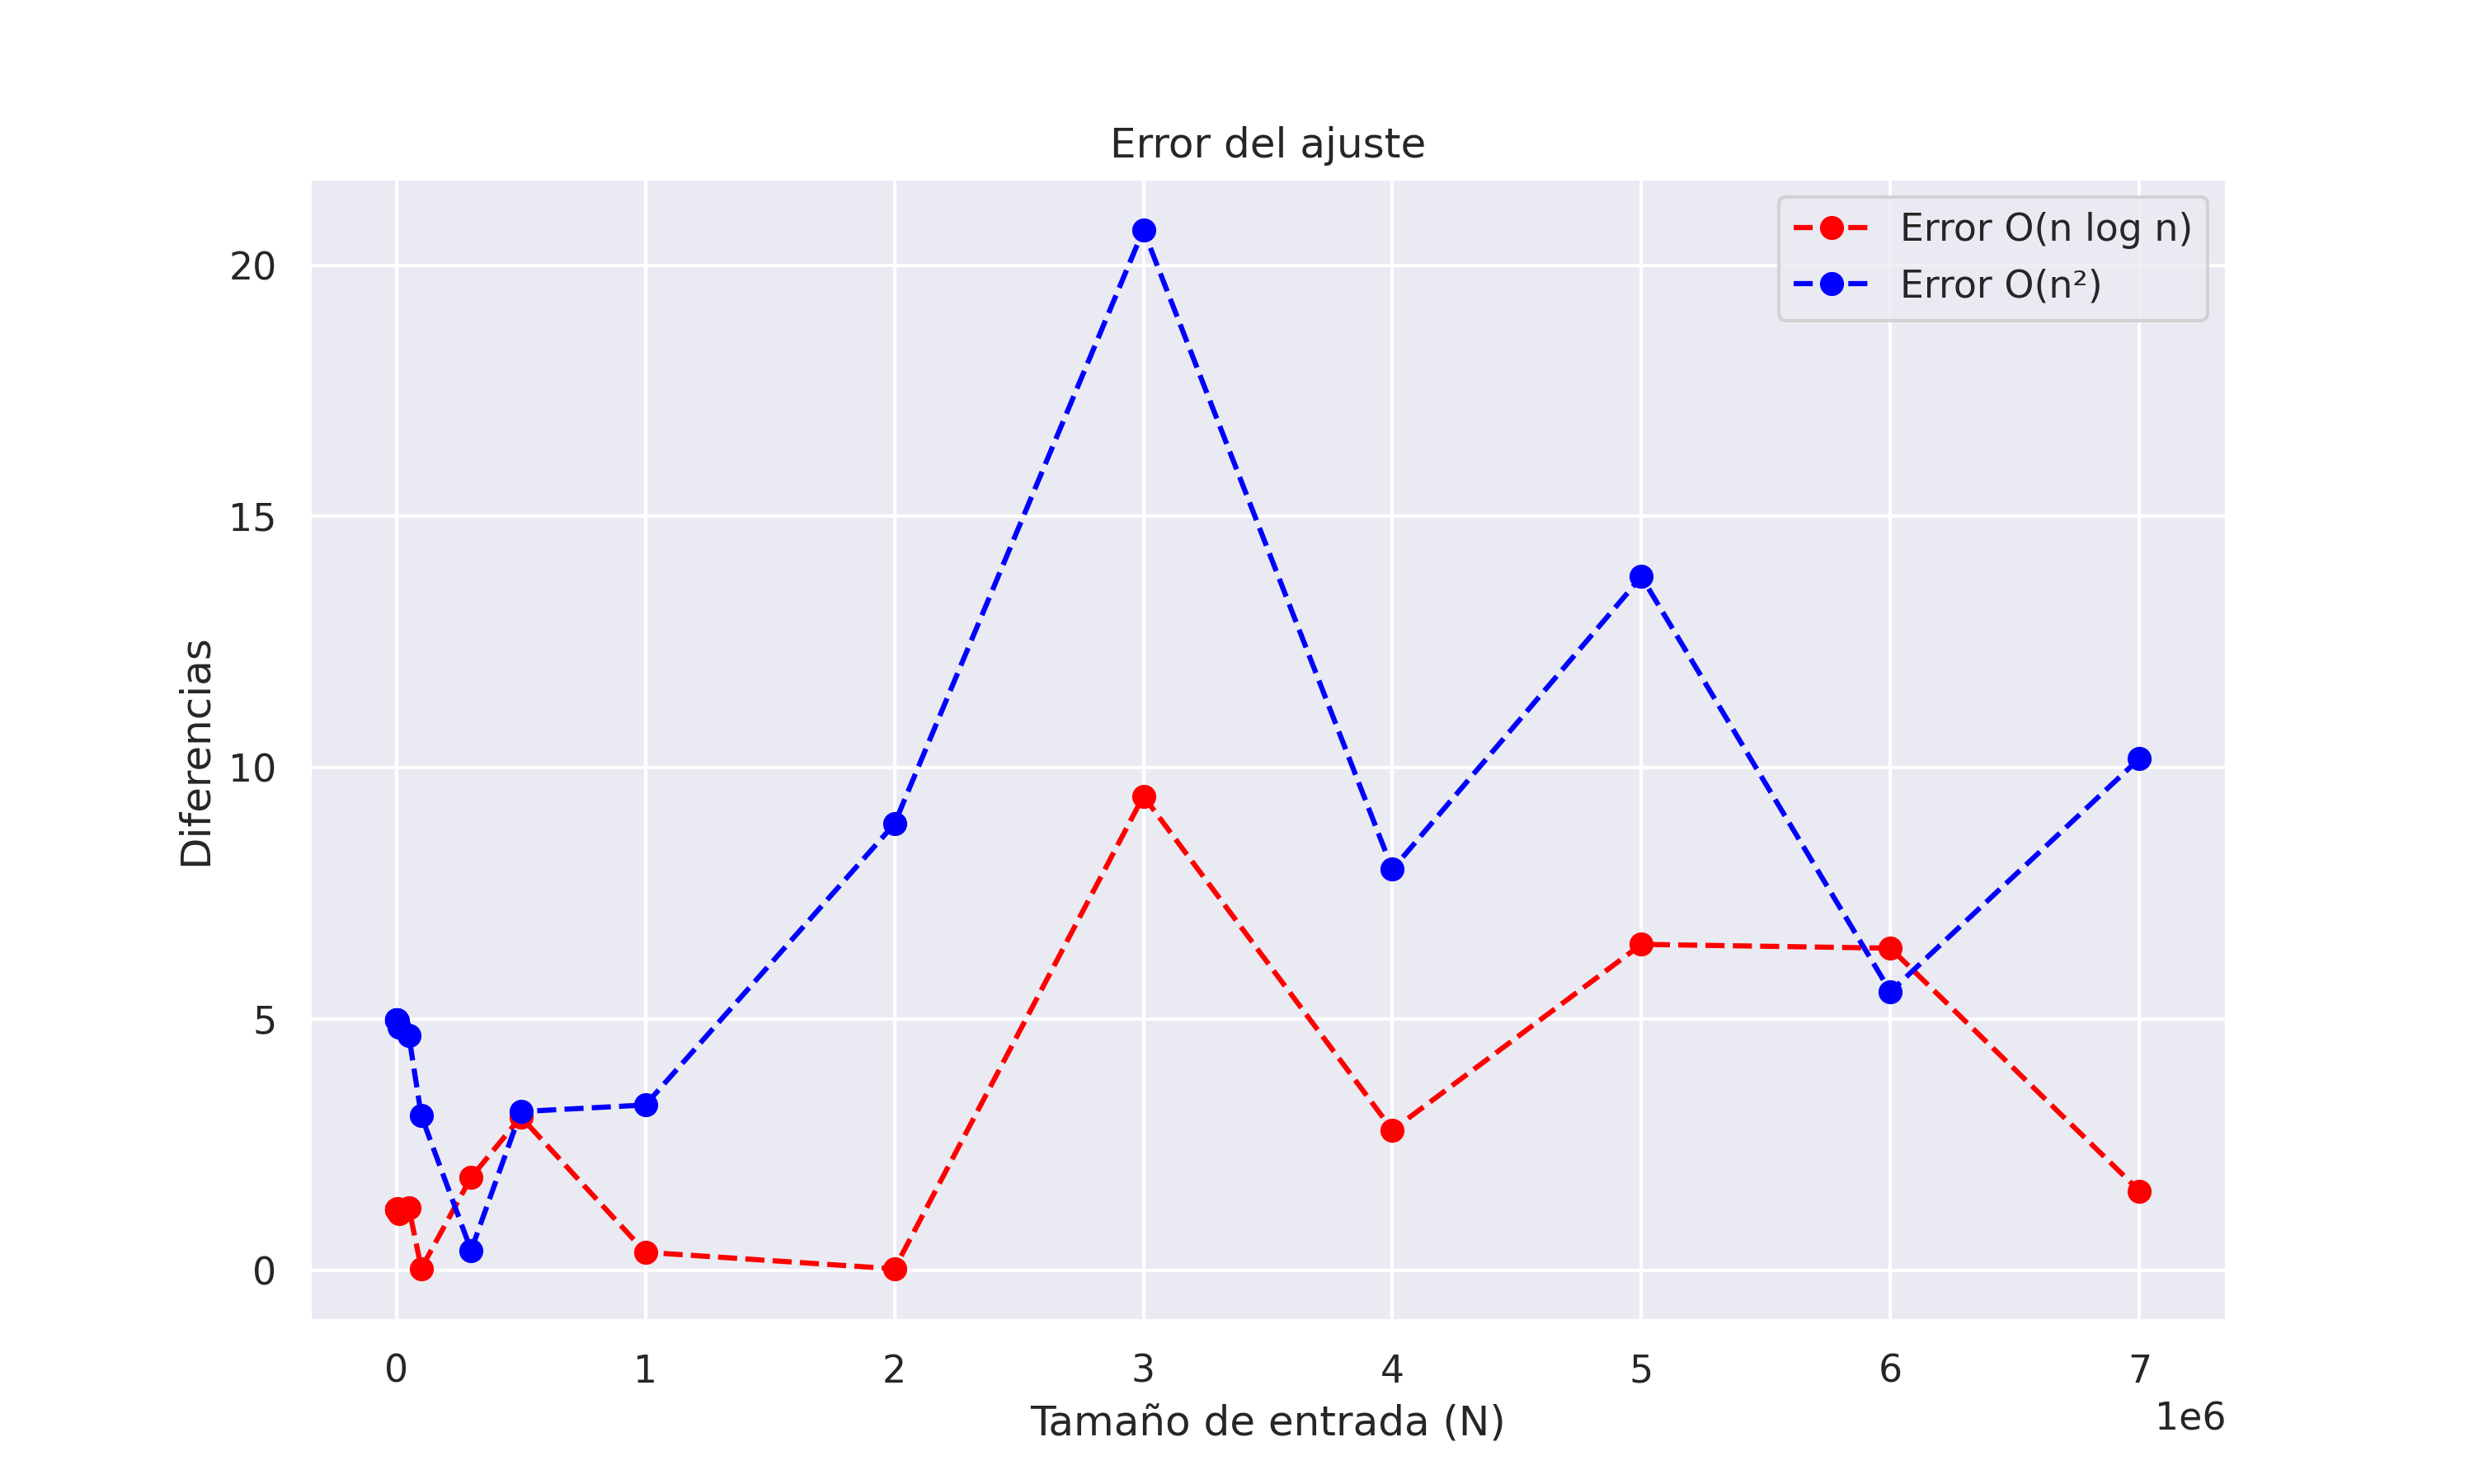
\includegraphics[width=1\textwidth]{img/error.png}
\end{figure}

notar, que en algunos datos el error de $O(n^2)$ es menor al de $O(nlogn)$, pero a nivel general, los datos se comporta mejor a la función de $O(nlogn)$.


Para obtener mas detalle de como correr los archivos y replicar el resultados, revisar el readme.md del repositorio.



%\section{Conclusiones}

Para encontrar la solución del problema, es importante destacar que en programación dinámica es necesario realizar un análisis previo del problema, siendo este el mayor problema del mismo. Teniendo en cuenta los algoritmos de Greedy que se tiene que elegir la decisión codiciosa que nos puede dar la mejor solución local en el estado correspondiente, en programación dinámica buscamos encontrar la mejor solución del estado actual definiendo mis variables de estados, de esta forma puedo guardar o memorizar los valores previos para poder ahorrar re calcular el mismo estado varias veces, además la programación dinámica nos permite explorar diferentes caminos para poder encontrar la mejor solución.

Es importante que reconstruir la solución tiene su complejidad que tenemos que asegurar que el tiempo que demore a lo sumo sea igual que encontrar la solución, en el caso que sea peor, seria mejor reconstruir el algoritmo porque encontrar la solución debería ser el algoritmo con mayor complejidad del problema.

Un punto extra es la medición de los tiempos del algoritmo, esto nos permite chequear que la teoría se corroborar con la practica realizada, usando métodos matemáticos que nos permiten buscar una función que mejor aproxima los puntos medidos desde un código aparte.
}


\newpage
\end{document}